\chapter{Avaliação}\label{chp:resultado}

\section{Introdução}\label{sec:resultado-introducao}
Neste capítulo apresentaremos um caso real de utilização da ferramenta como demonstração do resultado obtido no desenvolvimento deste projeto. Além disso, apresentaremos trabalhos relacionados a alternativas que visam facilitar a gestão de processos.

\section{Caso real}\label{sec:resultado-caso_real}

Em um cliente da Visagio, onde o Redmine já era utilizado para a gestão de diversos processos na área de Suprimentos, observou-se a necessidade da implantação de fluxos de aprovação mais complexos do que o Redmine poderia oferecer por padrão. Nesse cenário, observamos uma excelente oportunidade para avaliar na prática o funcionamento da solução descrita ao longo deste trabalho.

A Figura \ref{fig:process_cartao_compras} demonstra o processo para solicitação de criação de cartão de crédito corporativo. Este processo foi configurado para ser conduzido no Activiti BPM e Redmine através do plugin do Redmine \textit{BPM Integration} desenvolvido neste trabalho. O processo pode ser criado pelo funcionário que precisa utilizar um cartão, ou pelo seu superior, que abrirá em seu lugar. O processo é disparado mediante a abertura de um chamado no Redmine, onde são preenchidos dados pessoais do solicitante, endereço para entrega do cartão e diretor aprovador. Após a criação do processo, o Activiti BPM imediatamente cria a próxima tarefa: \textit{Workflow Diretor}. Através do mecanismo de sincronização, uma sub-tarefa é criada no Redmine, representando a aprovação do diretor. Esta tarefa tem o responsável definido pelo preenchimento do aprovador na tarefa anterior, sendo encaminhado através do fluxo no Activiti BPM ao Redmine definindo o responsável pela tarefa. Como é possível observar no diagrama, o processo segue por mais um nível de aprovação a ser executado pelo Normativo, área que é responsável por validar as informações preenchidas. Após aprovado, o processo segue para emissão, representada pela etapa \textit{Workflow Banco}, a ser realizada pelo atendente do banco, que concluirá a mesma assim que o cartão for emitido e enviado ao solicitante. Caso algum dos aprovadores reprove a solicitação do cartão, o chamado é encerrado e assume o status Reprovado.

\begin{figure}[H]
\centering
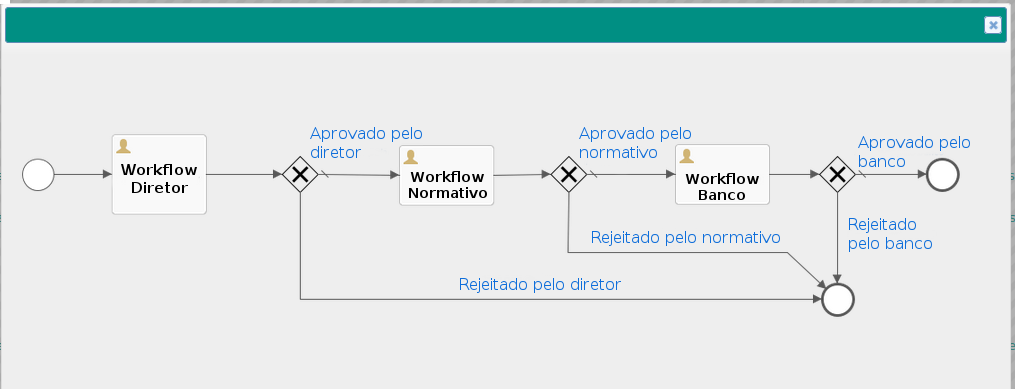
\includegraphics[width=1\textwidth]{imagens/process_criacao_cartao_corporativo.png}
\caption{Modelo de processo de criação de cartão corporativo}
\label{fig:process_cartao_compras}
\end{figure}

No caso do processo descrito, a implementação no Activiti BPM permitiu que as tarefas de aprovação fossem atribuídas automaticamente, e que a reprovação de uma etapa resultasse no encerramento do processo com o status Reprovado. Esse comportamento não seria possível de maneira simples no Redmine, diferentemente do Activiti BPM, onde a modelagem permite esse tipo de fluxo de trabalho.

No mês seguinte a primeira experiência do uso da integração entre o Redmine e o BPMS, novos processos foram implantados utilizando a mesma solução, dessa vez para orquestrar fluxos de cadastro de fornecedores da companhia. A Figura \ref{fig:processo_cadastro_fornecedores} representa a modelagem de um desses fluxos, em que é necessária a aprovação da área normativa do processo da empresa antes que o cadastro seja realizado.

\begin{figure}[H]
\centering
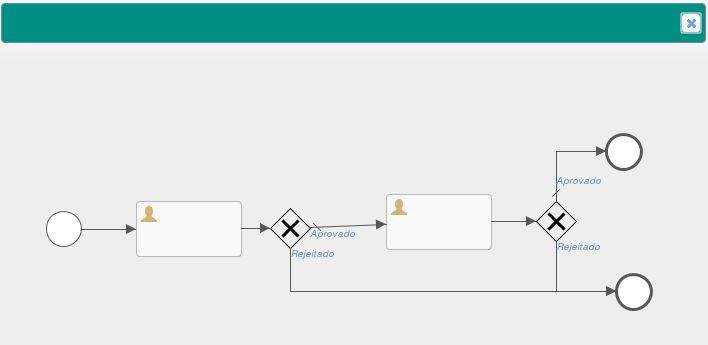
\includegraphics[width=1\textwidth]{imagens/processo_cadastro_fornecedores.png}
\caption{Modelo de processo de cadastro de fornecedores}
\label{fig:processo_cadastro_fornecedores}
\end{figure}

Por fim, após 6 meses de uso do \textit{plugin} objeto deste trabalho para o processo de cadastro de fornecedores, um novo e mais complexo grupo de processos foi incorporado à plataforma, o Recebimento Fiscal. As Figuras \ref{fig:processo_recebimento_fiscal_1} e \ref{fig:processo_recebimento_fiscal_2} ilustram o fluxo do processo de recebimento de Nota Fiscal de Serviços, que foi dividido em 2 partes para melhor visualização.

\begin{figure}[H]
\centering
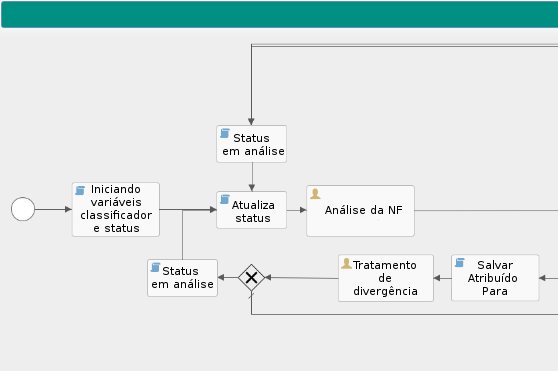
\includegraphics[width=1\textwidth]{imagens/processo_recebimento_fiscal(1).png}
\caption{Modelo de processo de recebimento fiscal (Parte 1)}
\label{fig:processo_recebimento_fiscal_1}
\end{figure}

\begin{figure}[H]
\centering
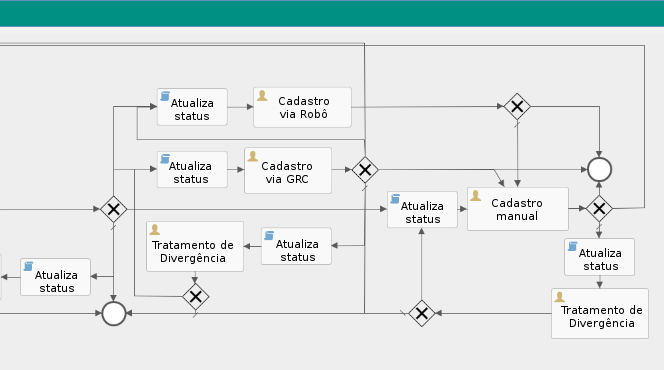
\includegraphics[width=1\textwidth]{imagens/processo_recebimento_fiscal(2).png}
\caption{Modelo de processo de recebimento fiscal (Parte 2)}
\label{fig:processo_recebimento_fiscal_2}
\end{figure}

Este processo inclui desde o envio da nota fiscal pelo fornecedor, passando pela validação de seus dados pelos analistas da área de recebimento fiscal e tratamento de possíveis inconsistências encontradas, até o cadastro da nota no ERP\cite{erp_definition} (\textit{Enterprise Resource Planning}) da empresa. 

Este processo envolve vários atores responsáveis pelas diferentes etapas do processo, e a distribuição das tarefas entre eles é feita automaticamente pela camada de integração desenvolvida.

No gráfico da Figura \ref{fig:grafico_processo} é possível verificar o total de processos iniciados (Abertos) e concluídos (Fechados) para os três diferentes grupos de processos. Ao observarmos que todos os processos tem um alto percentual de conclusão, podemos concluir que a integração entre o Redmine e o Activiti BPM funcionou conforme o esperado, e que os processos fluíram normalmente com a interação dos atores do processo através do Redmine. Além disso, não foram observados reclamações importantes referentes ao funcionamento do fluxo de trabalho. No total, foram iniciados 70.162 processos desde Março de 2016, o que representa uma média de 220 processos iniciados por dia até Janeiro de 2017.

\begin{figure}[H]
\centering
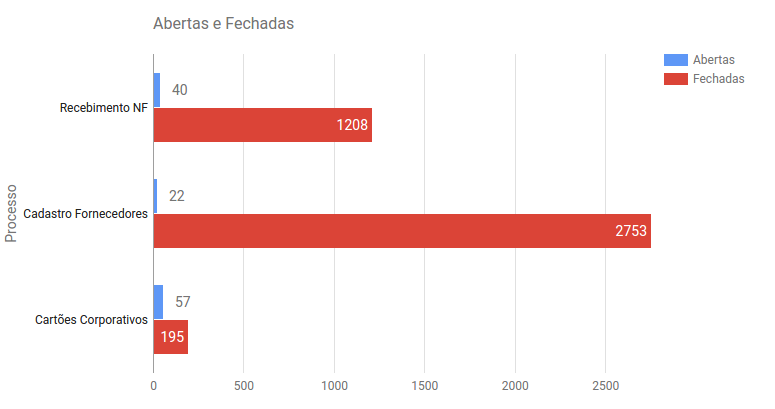
\includegraphics[width=1\textwidth]{imagens/grafico_processo.png}
\caption{Processos utilizando o plugin}
\label{fig:grafico_processo}
\end{figure}

\section{Trabalhos relacionados}\label{sec:resultado-relacionados}

A seguir são apresentados alguns trabalhos relacionados ao tema central deste trabalho, que é a utilização de metodologias e ferramentas com objetivo de facilitar e otimizar a gestão e execução de processos.

\subsection{Melhoria de processos pelo BPM: aplicação no setor público}\label{subsec:resultado-relacionados-caso_setor_publico}
Este artigo \cite{artigo_relacionado_setor_publico} apresenta um relato de aplicação da metodologia BPM, que foi adaptada para o contexto de uma organização pública e utilizada para modernizar o processo de controle de trânsito animal no Brasil. A partir da análise do processo atual foram propostas melhorias a fim de otimizar recursos, melhorar a confiabilidade e aumentar a satisfação de clientes.

\subsection{JIRA Core}

JIRA Software\cite{jira-software} é um sistema de gestão de projetos de \textit{software} que é utilizado para realizar a gestão de erros, melhorias e novas funcionalidades, utilizando fluxos de trabalho personalizados de acordo com a necessidade de cada projeto, como o Redmine.

No entanto, foi percebido pelos responsáveis da ferramenta o seu uso crescente para projetos não técnicos\cite{jira-core-guide}, fugindo do público alvo original. Então, para suprir a necessidade desses times foi criado o JIRA Core\cite{jira-core}, que é um \textit{software} de gestão de processos de negócio que permite a configuração de diferentes fluxos de trabalho pelos usuários administradores do próprio sistema e fornece mecanismos de controle e acompanhamento da execução desses processos.

A abordagem do JIRA Core foi diferente da proposta deste trabalho. Aquele buscou embutir nele mesmo, principalmente, a configuração de fluxos de processos simples, porém ainda mais complexos do que o JIRA Software permitia. O plugin \textit{BPM Integration}, por sua vez permitiu a configuração de fluxos complexos através da integração do Redmine com o BPM.